\section{Basics of gradient-based edgedetection}

\begin{frame}
	\frametitle{One dimensional approach}
	\begin{center}
		\begin{figure}
			\centering
			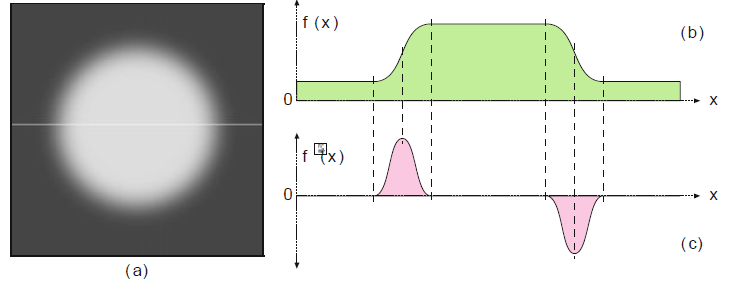
\includegraphics[width=0.7\linewidth]{images/1DGradient}
			\caption[1D Gradient]{One dimensional image function and derivation}
			\label{fig:1dgradient}
		\end{figure}
		\b{Only applyable with known, steady functions}
	\end{center}
\end{frame}

\begin{frame}
	\frametitle{Approximating discrete derivation}
	Problem: the image function is discrete, therefore we need to approximate the derivation
	\begin{center}
		\begin{figure}
			\centering
			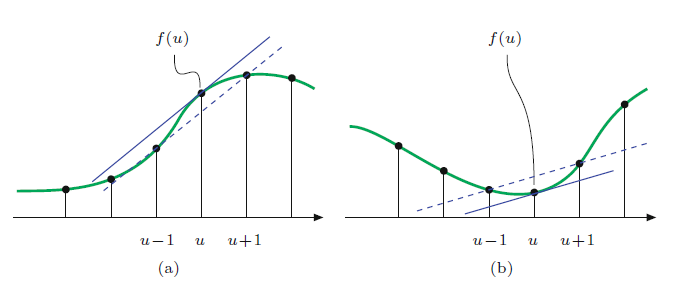
\includegraphics[width=0.7\linewidth]{images/1DGradientApproximation}
			\caption[1D Gradient Approximation]{Approximation of the derivation for discrete imagefunctions}
			\label{fig:1dgradientapprox}
		\end{figure}
		$\dfrac{df}{dx}(u) \approx \dfrac{f(u+1) - f(u-1)}{(u+1)-(u-1)} = \dfrac{f(u+1) - f(u-1)}{2}$
	\end{center}
\end{frame}

\begin{frame}
	\frametitle{Two dimensional approach}
	If working with full images,we got two dimensions and therefore two partial derivations:
	\begin{center}	
		$I_x = \dfrac{\partial I}{\partial x}(u,v) , I_y = \dfrac{\partial I}{\partial y}(u,v)$
	\end{center}
	the \textbf{gradient} at the point \textit{(u,v)} is \newline
	\begin{center}
		$\nabla I(u,v) =  \begin{pmatrix}I_x(u,v) \\ I_y(u,v)\end{pmatrix}$
	\end{center}	
	~\newline
	And the \textbf{magnitude} is \newline
	\begin{center}
		$|\nabla I|=\sqrt{I_x^2 + I_y^2}$
	\end{center}
\end{frame}

\begin{frame}
	\frametitle{Example}
	\begin{figure}
		\centering
		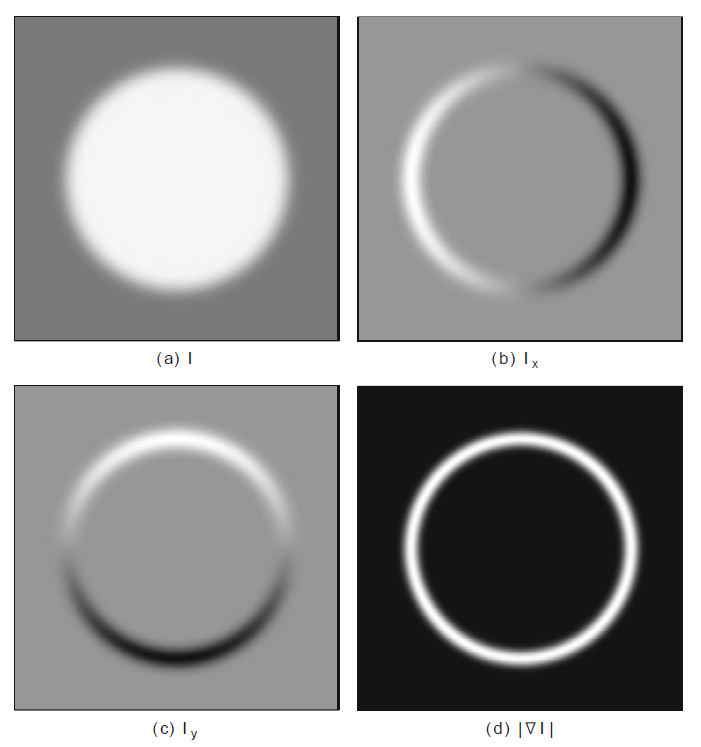
\includegraphics[width=0.5\linewidth]{images/2DEdgeGradient}
		\caption{Visualisation of simple gradient-based edgedetection}
		\label{fig:2dedgegradient}
	\end{figure}
\end{frame}

\begin{frame}
	\frametitle{Example with Felix}
	\begin{figure}
		\centering
		\begin{subfigure}[b]{0.175\textwidth}
			\centering
			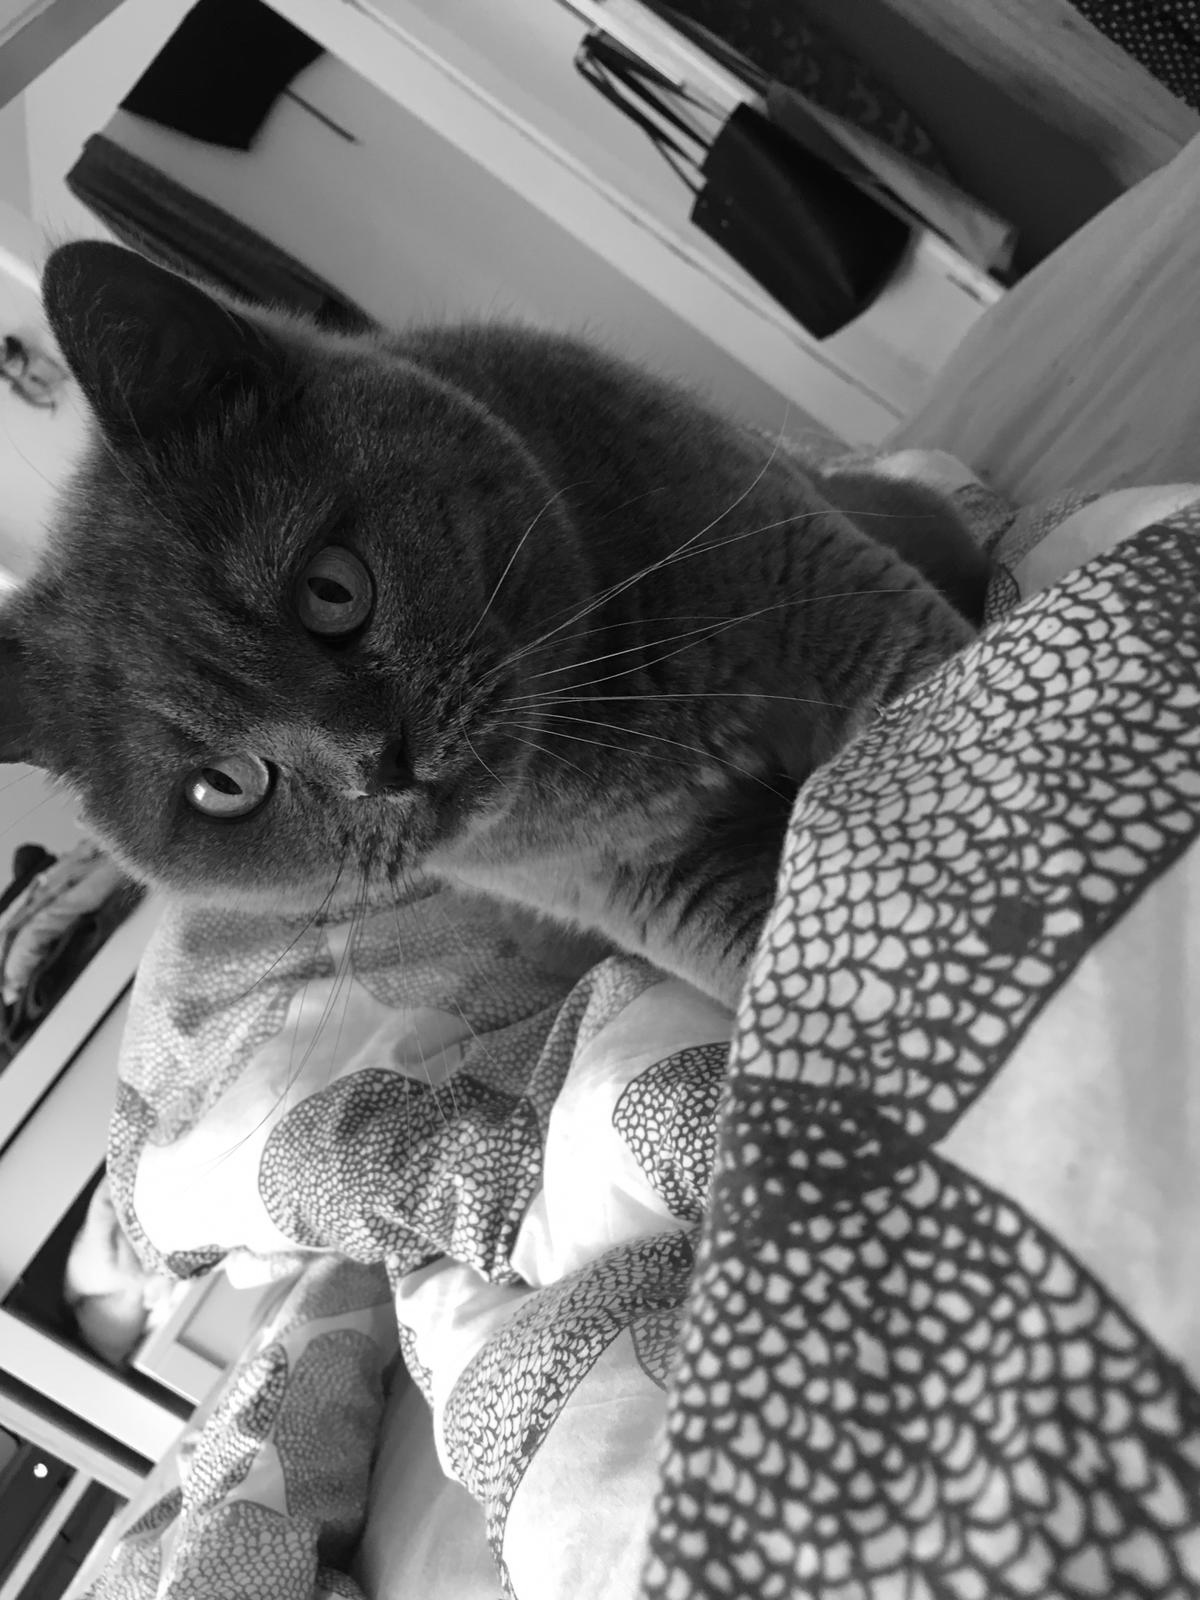
\includegraphics[width=\textwidth]{images/Kadse}
			\caption[I]%
			{{\small I}}    
			\label{fig:RawFelix}
		\end{subfigure}
		\quad
		\begin{subfigure}[b]{0.175\textwidth}  
			\centering 
			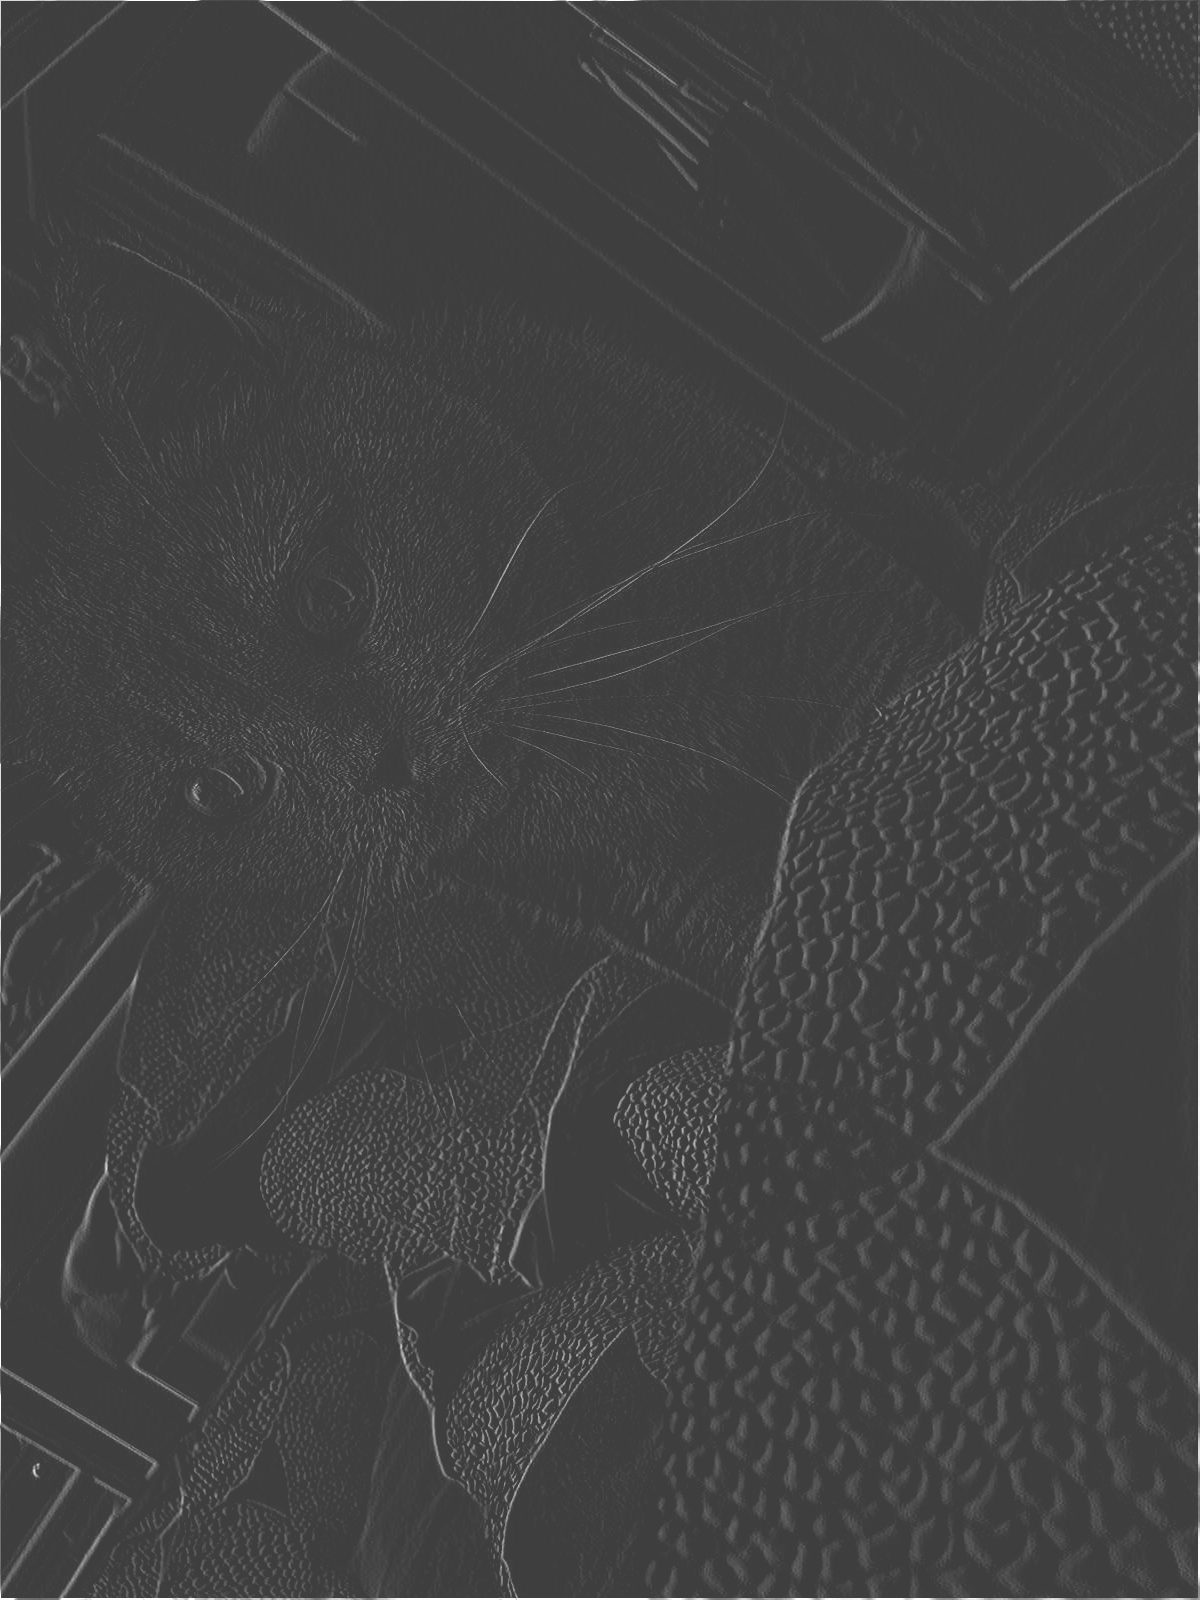
\includegraphics[width=\textwidth]{images/KadseSimpleX}
			\caption[]%
			{{\small $I_x$}}    
			\label{fig:FelixX}
		\end{subfigure}
		\vskip\baselineskip
		\begin{subfigure}[b]{0.175\textwidth}   
			\centering 
			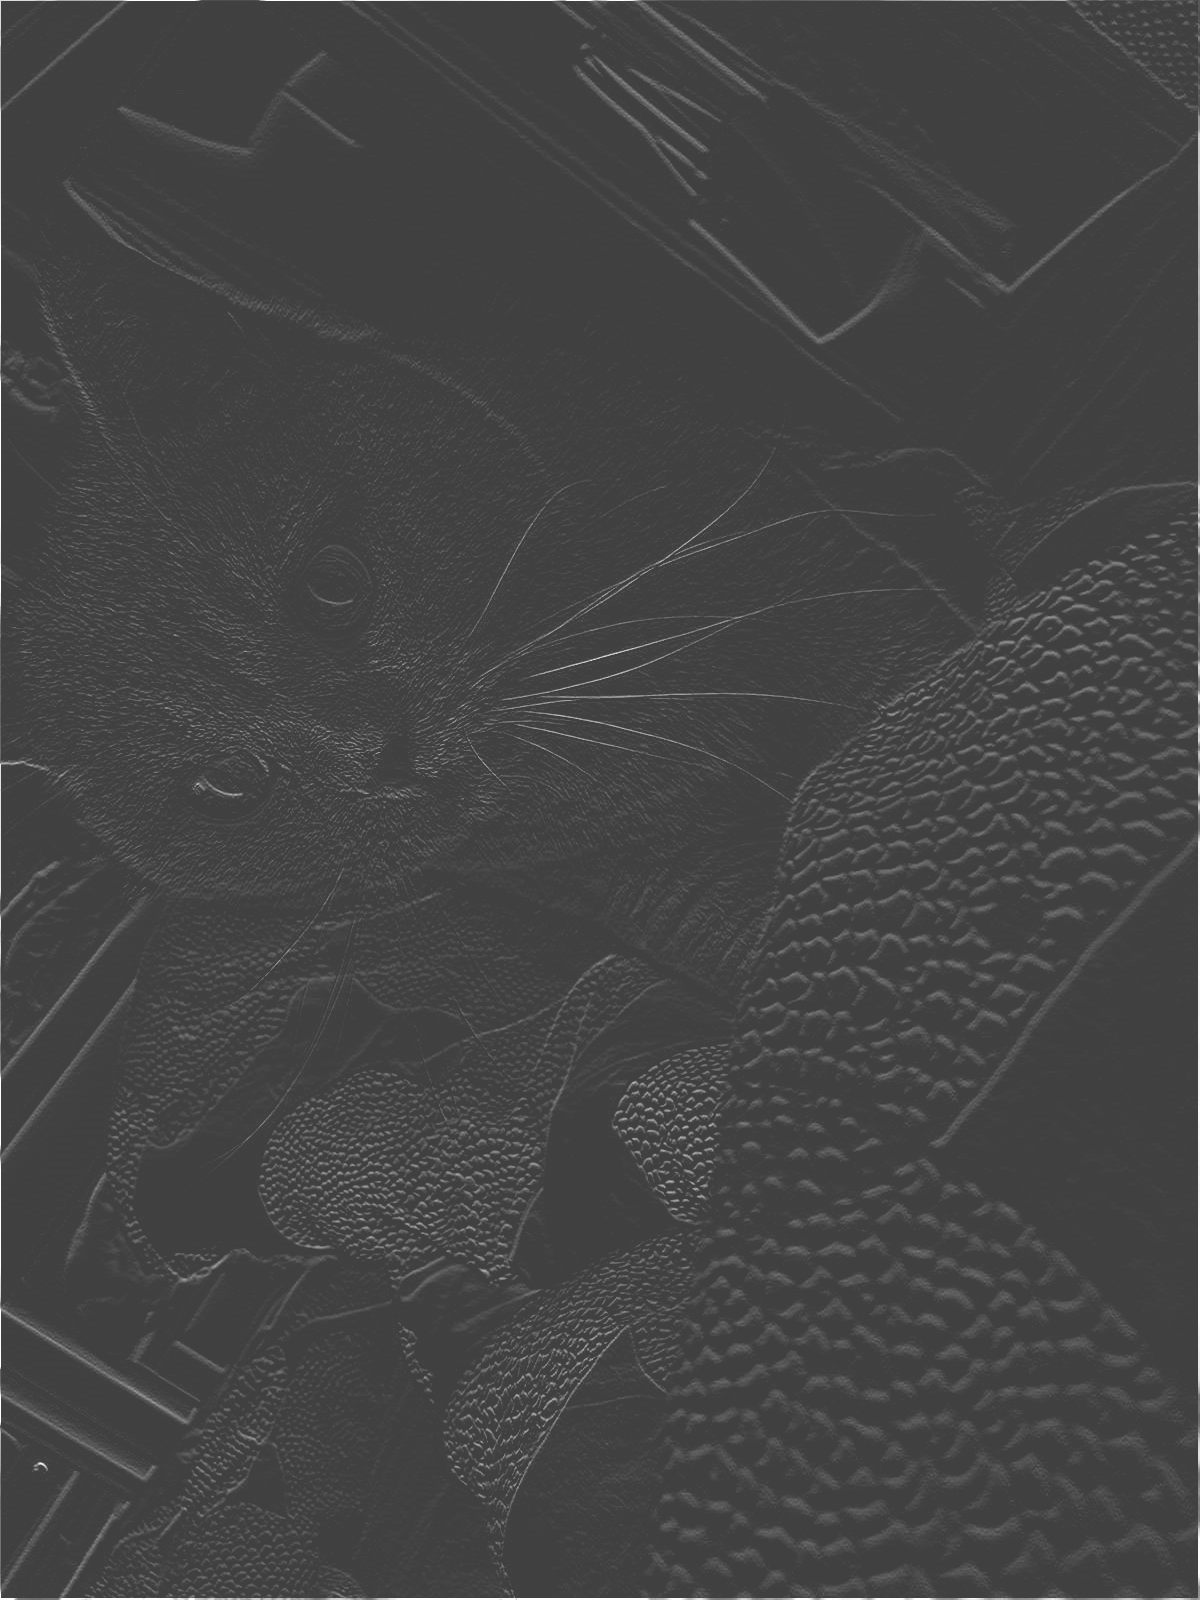
\includegraphics[width=\textwidth]{images/KadseSimpleY}
			\caption[]%
			{{\small $I_y$}}    
			\label{fig:FelixY}
		\end{subfigure}
		\quad
		\begin{subfigure}[b]{0.175\textwidth}   
			\centering 
			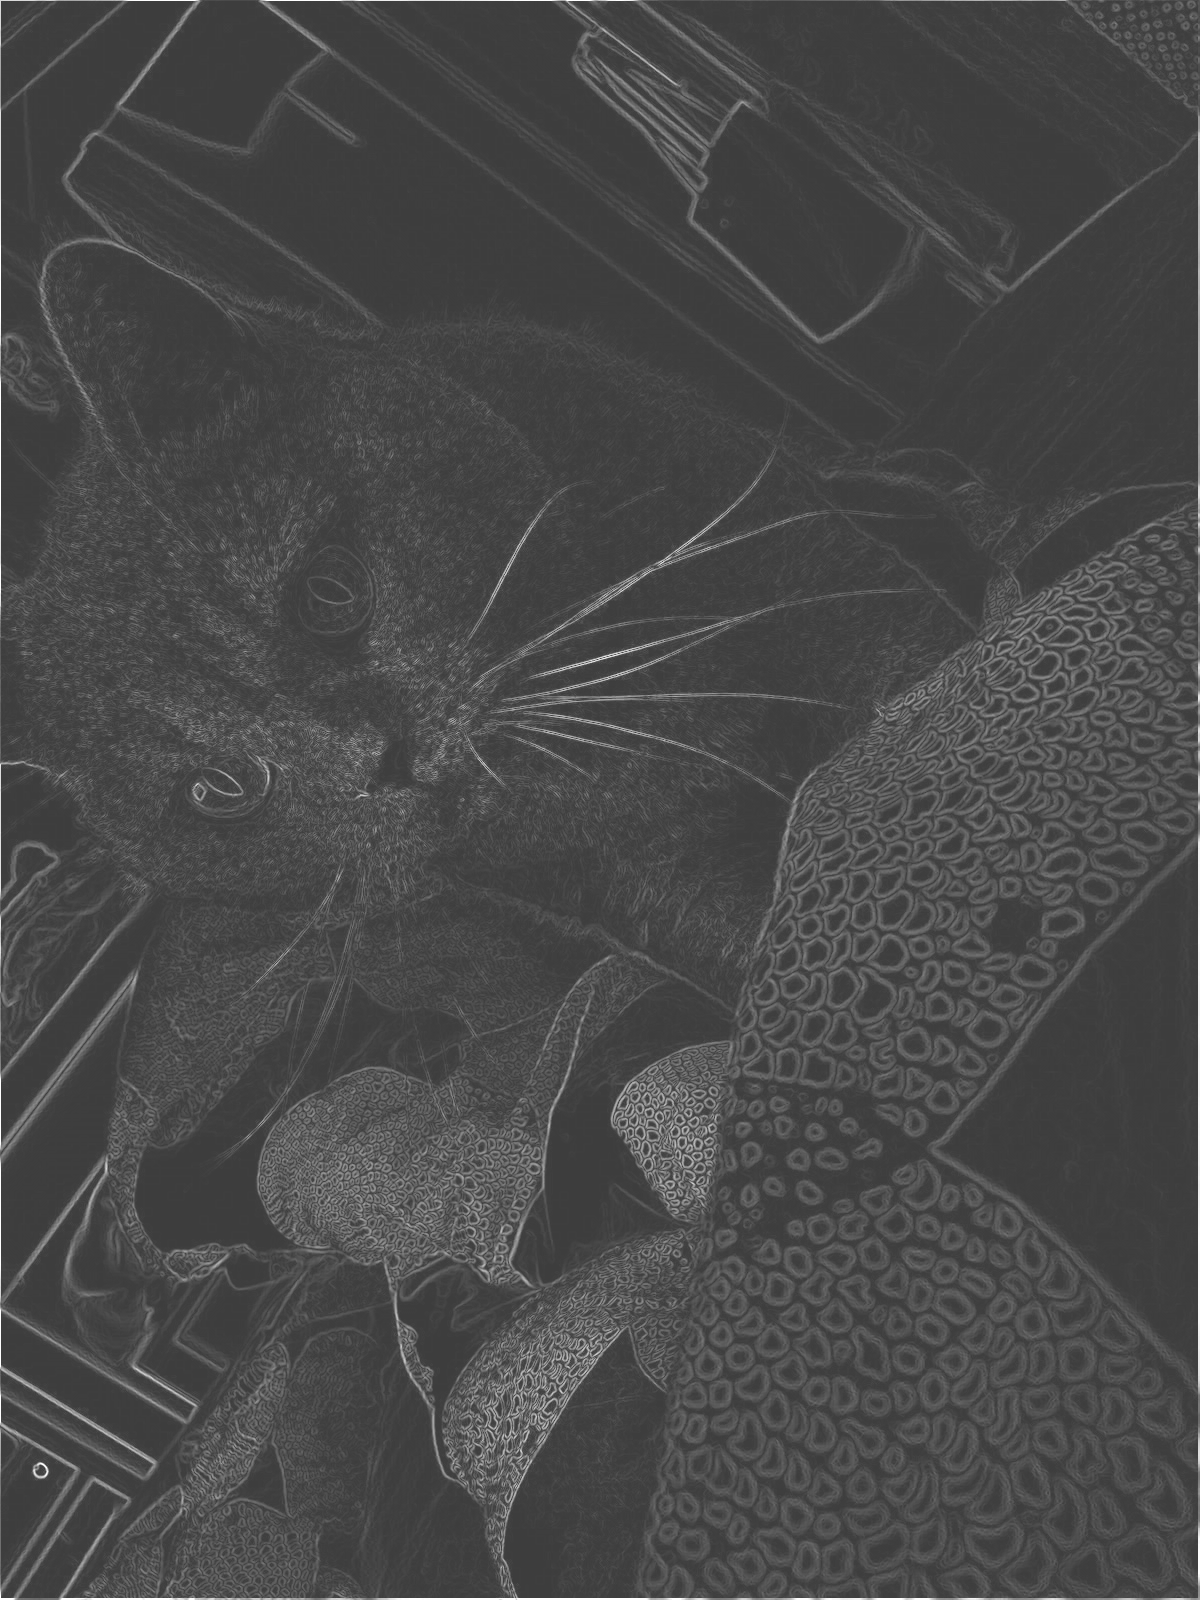
\includegraphics[width=\textwidth]{images/KadseSimple}
			\caption[]%
			{{\small $|\nabla I |$}}    
			\label{fig:FelixSimple}
		\end{subfigure}
		\caption[Simple Filters applied to Felix ]
		{\small Simple Filters applied to Felix\footnote{All images have a 50\% increased brightness}} 
		\label{fig:FullSimpleFelix}
	\end{figure}
	
	
\end{frame}
\begin{frame}
	\frametitle{Implementation with filters}
	\label{SimpleFilters}
	Expressing the gradient as a \textit{linear filter} is simple:
	\begin{columns}
		\begin{column}{0.5\textwidth}
			\begin{center}
				$I_x = \begin{bmatrix} -0.5 & 0 & 0.5\end{bmatrix}$
			\end{center}	
		\end{column}
		\begin{column}{0.5\textwidth} 
			\begin{center}
				$I_y = \begin{bmatrix} -0.5 \\ 0 \\ 0.5\end{bmatrix}$
			\end{center}
		\end{column}
	\end{columns}
\end{frame}
